\clearpage
\section{Architettura del sistema}
L'architettura del sistema è stata formalizzata attraverso due \textit{deployment diagram} differenti: il primo, riportato in figura \ref{fig:DeplymnetDiagramNonFormale}, rappresenta il sistema tramite una notazione a stile libero, mentre il secondo, riportato in figura \ref{fig:DeplymnetDiagramFormale}, rappresenta il sistema tramite lo stile UML. In particolare, in entrambi i diagrammi è possibile identificare un pattern architetturale \textit{three-tier}. 
Il \textit{presentation layer} è costituito dalle applicazioni lato client che vengono utilizzate dagli utenti. Nell'\textit{application layer}, invece, ci sono due sistemi distinti:

\begin{itemize}
	\item l'applicativo \textbf{LVSEmergency}, che si occupa della gestione di richieste HTTP/REST che permettono l'interazione con il client;
	\item due componenti autonome: un \textbf{Data Collector} che si occupa di recuperare informazioni dai \textit{data server} tramite API REST e le inserisce all'interno del database presente nel \textit{data layer}, ed un \textbf{Data Analyzer} che si occupa di effettuare delle analisi sui dati acquisiti con lo scopo di identificare possibili situazioni di allarme. È bene notare che queste due applicazioni non costituiscono una vera e propria \textit{Big Data Pipeline} in quanto vengono effettuate solo la collezione e l'analisi dei dati raccolti. \todo{da controllare}
\end{itemize}

Nel \textit{data layer} troviamo invece un database all'interno del quale sono inseriti tutti i dati necessari per il funzionamento dell'applicazione.

\begin{landscape}
	\begin{figure}[b]
		\centering
		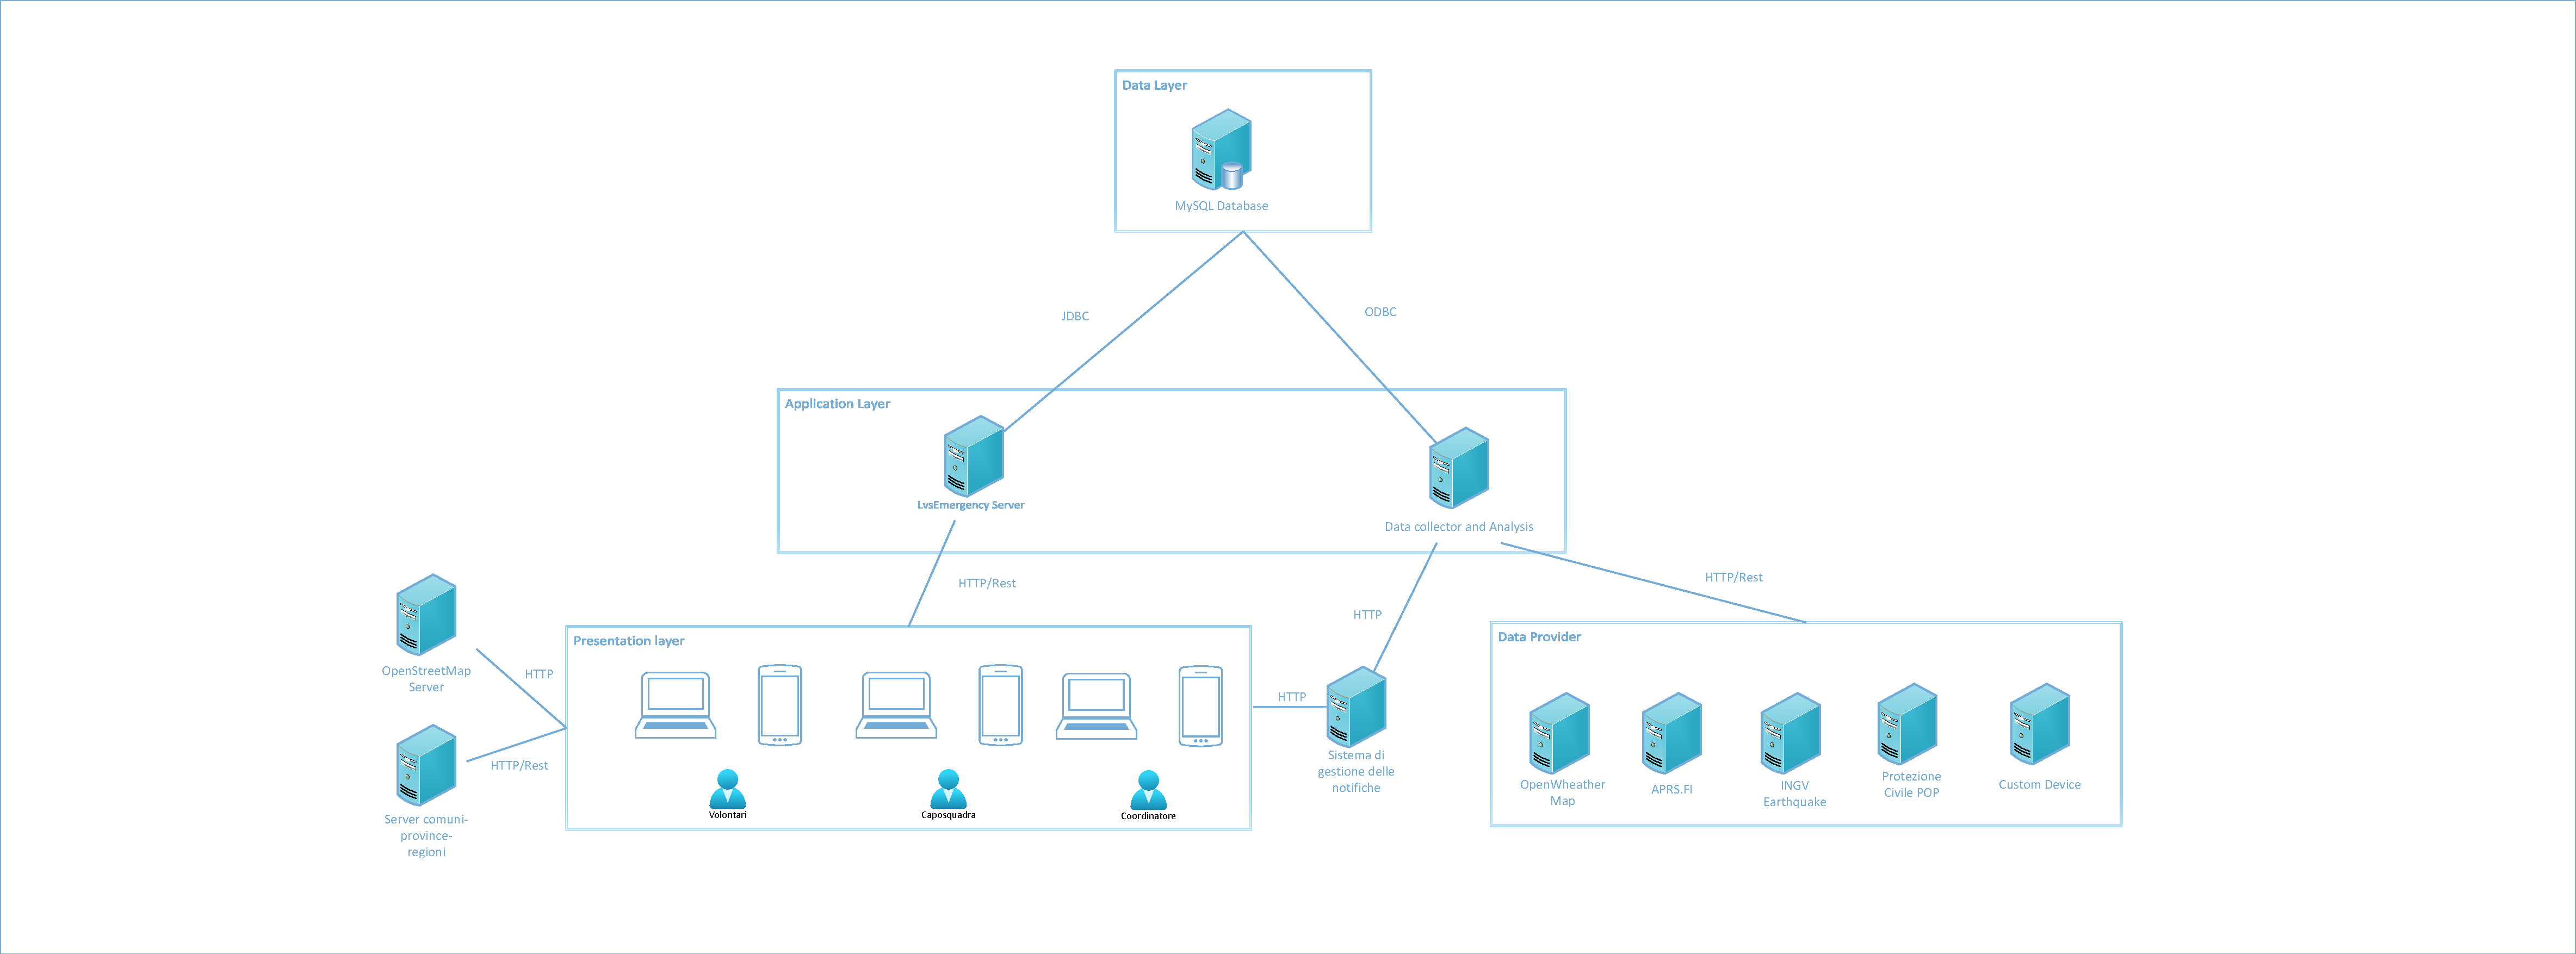
\includegraphics[width=1.1\linewidth]{./Iterazione 0/OtherFiles/DeploymentDiagramNonFormale}
		\caption{Deployment diagram in stile libero.}
		\label{fig:DeplymnetDiagramNonFormale}
	\end{figure}
\end{landscape}
\begin{landscape}
	\begin{figure}[b]
		\centering
		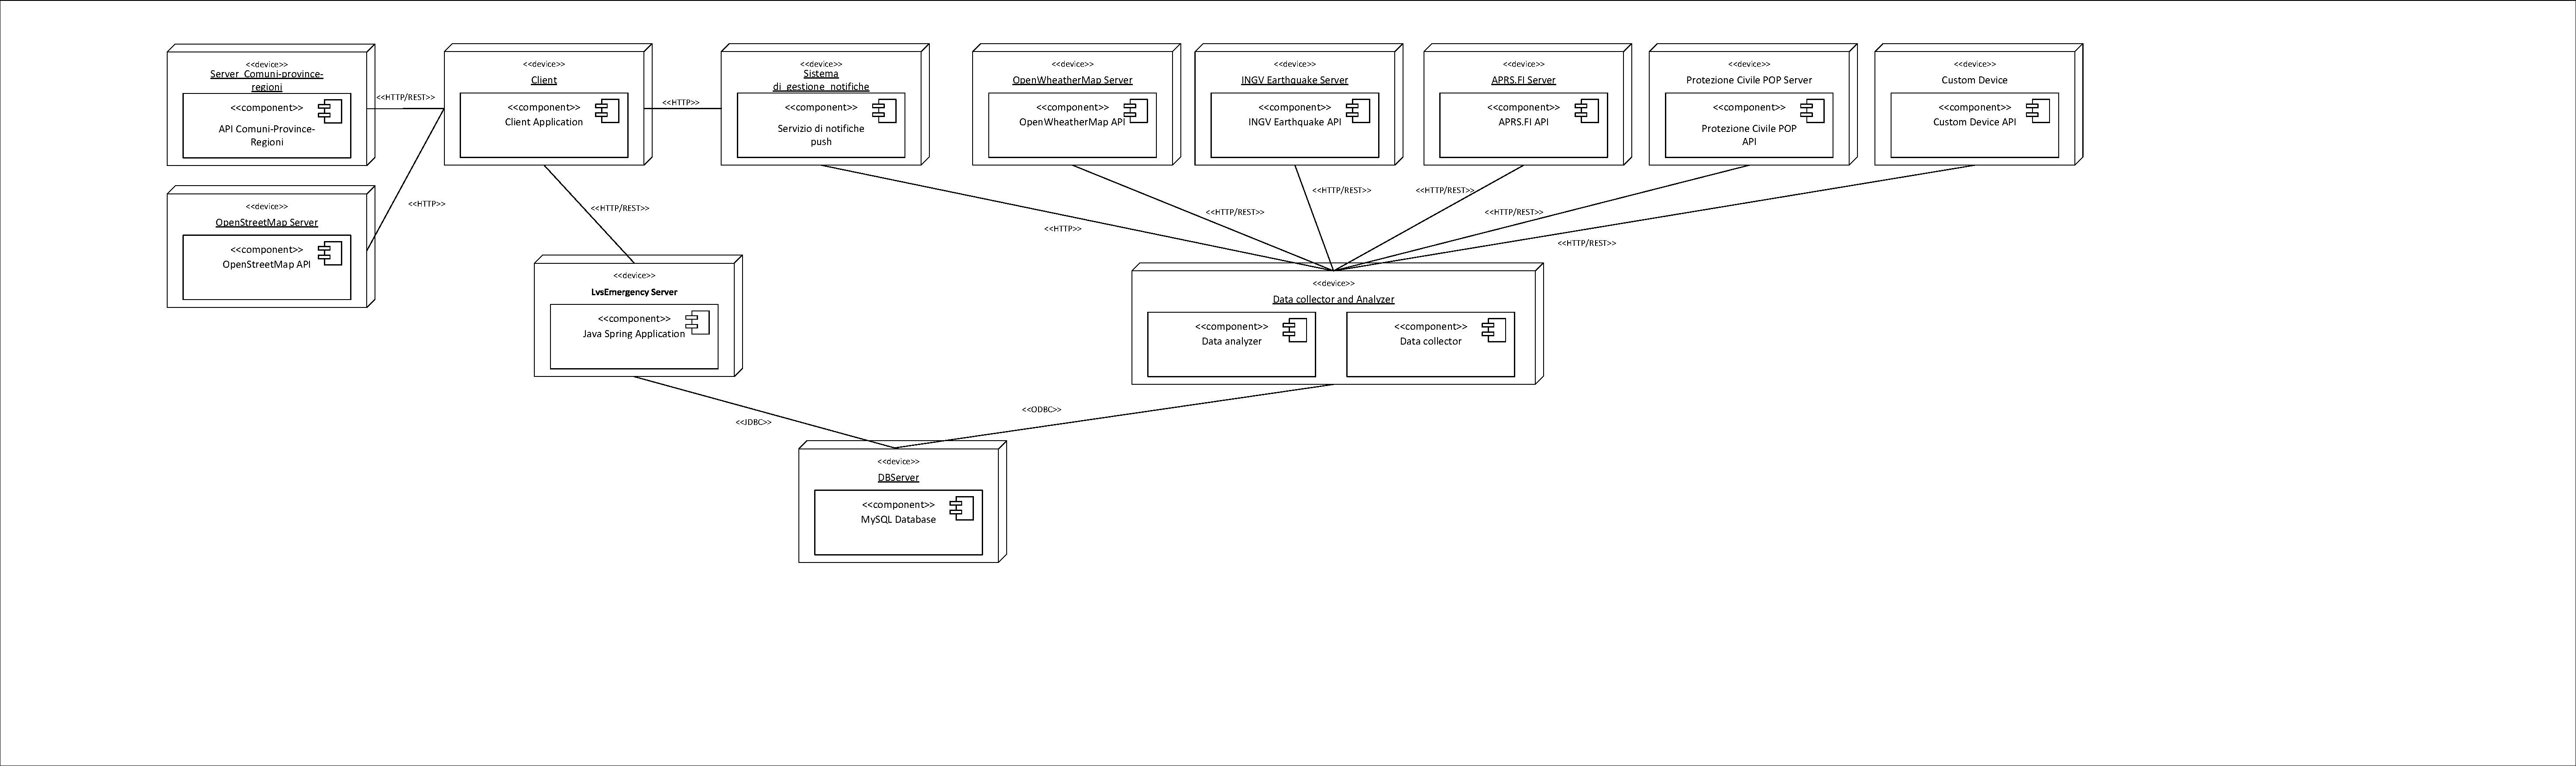
\includegraphics[width=1.1\linewidth]{./Iterazione 0/OtherFiles/DeplymentDiagramFormale}
		\caption{Deployment diagram in stile UML.}
		\label{fig:DeplymnetDiagramFormale}
	\end{figure}
\end{landscape}
